\documentclass[border=10pt]{standalone}
\usepackage{tikz}
\usetikzlibrary{shapes.geometric, arrows.meta, positioning}

% Define flowchart styles
\tikzstyle{startstop} = [
    rectangle, 
    rounded corners, 
    minimum width=3cm, 
    minimum height=1cm,
    text centered, 
    draw=black, 
    fill=red!30,
    font=\bfseries
]

\tikzstyle{io} = [
    trapezium, 
    trapezium left angle=70, 
    trapezium right angle=110, 
    minimum width=3cm, 
    minimum height=1cm, 
    text centered, 
    draw=black, 
    fill=blue!30
]

\tikzstyle{process} = [
    rectangle, 
    minimum width=3cm, 
    minimum height=1cm, 
    text centered, 
    draw=black, 
    fill=orange!30
]

\tikzstyle{decision} = [
    diamond, 
    minimum width=3cm, 
    minimum height=1cm, 
    text centered, 
    draw=black, 
    fill=green!30,
    aspect=2
]

\tikzstyle{arrow} = [thick,->,>=Stealth]

\begin{document}

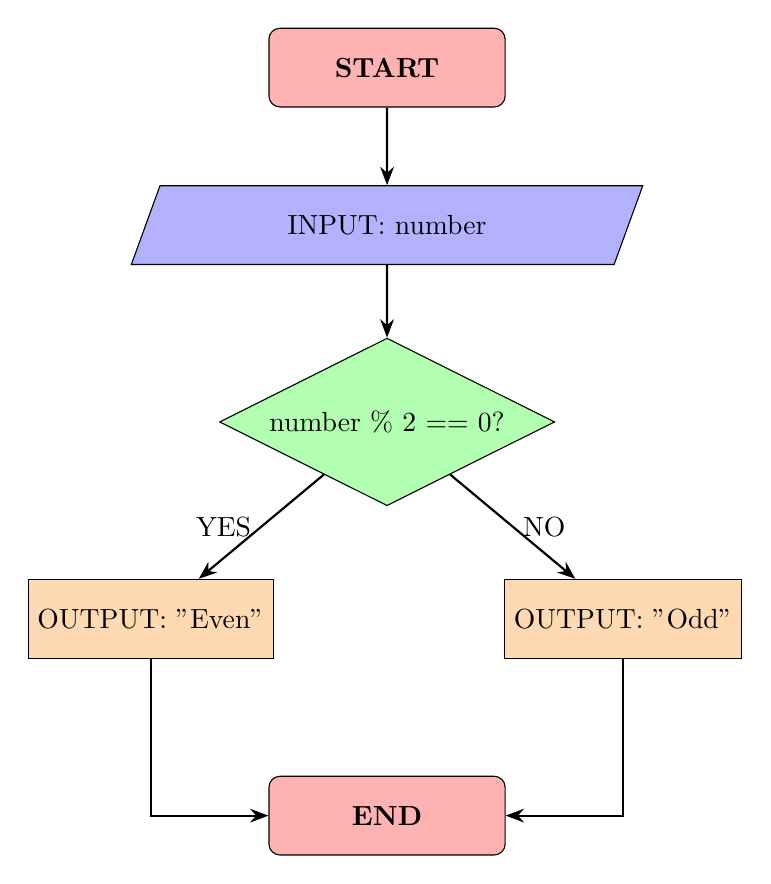
\begin{tikzpicture}[node distance=2cm]

% Nodes
\node (start) [startstop] {START};
\node (input) [io, below of=start] {INPUT: number};
\node (decision) [decision, below of=input, yshift=-0.5cm] {number \% 2 == 0?};
\node (even) [process, below of=decision, xshift=-3cm, yshift=-0.5cm] {OUTPUT: "Even"};
\node (odd) [process, below of=decision, xshift=3cm, yshift=-0.5cm] {OUTPUT: "Odd"};
\node (end) [startstop, below of=decision, yshift=-3cm] {END};

% Arrows
\draw [arrow] (start) -- (input);
\draw [arrow] (input) -- (decision);
\draw [arrow] (decision) -- node[anchor=east] {YES} (even);
\draw [arrow] (decision) -- node[anchor=west] {NO} (odd);
\draw [arrow] (even) |- (end);
\draw [arrow] (odd) |- (end);

\end{tikzpicture}

\end{document}